\chapter{Link lag}

\section{Opgaveformulering}

Til dette lag skal I implementere en modificeret SLIP protokol.
Protokollen skal implementeres således: Som start og stop karakter benyttes ’A’. Hvis karakteren ’A’ forekommer i telegrammet erstattes det med de to tegn ’B’ og ’C’, og hvis tegnet ’B’ forekommer, erstattes det med de to tegn ’B’ og ’D’.

\begin{figure}[htbp]
\centering
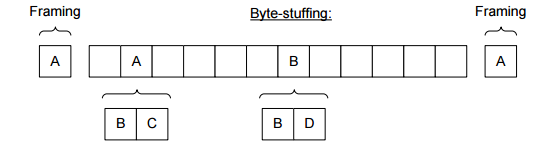
\includegraphics[width=1\linewidth]{Subpages/Billeder/Linklag}
\caption{Linklag protokollen}
\label{fig:Linklag}
\end{figure}



